\chapter{\label{chap:chap2} Fundamentação Teórica}

Este capítulo apresentará alguns protocolos de comunicação e técnicas que servirão de apoio para o desenvolvimento deste TCC. 
Por fim, alguns trabalhos relacionados a área serão expostos, bem como o posicionamento deste trabalho perante aos demais.

\section{BGP}


O protocolo BGP está situado na quinta camada, a camada de aplicação, do modelo de referência TCP/IP \cite{tanenbaum2011redes}.
Abaixo, de forma sucinta, elencaremos algumas funcionalidades básicas do protocolo que embasarão o restante deste trabalho.

\begin{itemize}
    \item A responsabilidade deste protocolo é manter a troca de informações sobre roteamentos entre sistemas autônomos \cite{Rekhter:1995}.
    \item O roteador ao entrar na rede pela primeira vez deve-se conectar ao seu vizinho. Após a conexão estabelecida, os roteadores compartilham entre sí suas tabelas de roteamento \cite{Rekhter:1995}.
    \item Posteriormente, as atualizações nas tabelas dos roteadores dão-se de forma incremental à medida que as mudanças na rotas ocorrem \cite{Rekhter:1995}.
    \item Mensagens de \textit{keep alive} são trocadas periodicamente a fim de garantir conectividade entre os roteadores \cite{Rekhter:1995}.
\end{itemize}

\section{CoAP}

Especificado pela RFC-7252, o CoAP, protocolo de aplicação restrita, foi projetado para aplicações máquina-a-máquina
e tem como foco a transferência de documentos web entre nodos com recursos limitados em redes de baixa qualidade\cite{rfc7252}.

O modelo de interação cliente/servidor é o padrão adotado pelo CoAP, entretanto,
o fato do protocolo ter sido projetado para aplicações máquina-a-máquina faz com que os dispositivos comumente desempenhem o papel de cliente e servidor simultaneamente.

Quando mensagens CoAP de requisição e resposta são trocadas, estas devem conter o código do método ou código da resposta, respectivamente.
Além dos códigos, as mensagens podem conter outras informações, como o recurso que se deseja acessar e o tipo de mídia que se está transportando.
Por fim, um token é utilizado para que haja a correspondência entre requisição e resposta.

A Figura \ref{fig:fig4} ilustra uma solicitação entre cliente e servidor, na qual o cliente deseja obter a temperatura.
Analisando a troca de mensagens, notamos que o cliente envia uma solicitação não confirmável com token 0x74 e código GET para acessar o recurso temperatura no servidor.
O servidor por sua vez retorna o código de resposta 2.05, que indica sucesso, o mesmo token que recebeu na solicitação do cliente e o valor 22.5 C.

\begin{figure}[htb!]
    \centering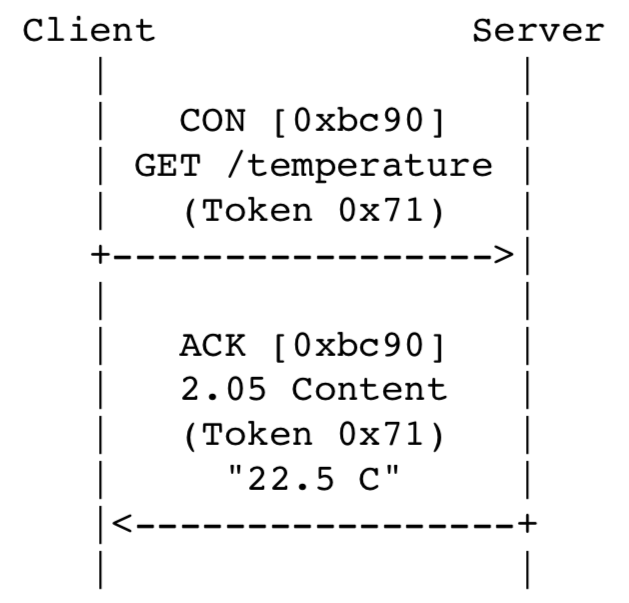
\includegraphics[height=.4\textwidth]{fig4.png} 
    \caption
    {\label{fig:fig4} Requisição e resposta utilizando mensagens não confirmáveis.} \cite{rfc7252}
\end{figure}

A arquitetura REST, assim como no protocolo HTTP\cite{rfc2616}, foi utilizada na projetização do protocolo CoAP.
Como ambos compartilham da mesma arquitetura, realizar o mapeamento de HTTP para CoAP e vice-versa é bastante simples.
Para realizar tal mapeamento basta utilizarmos o \textit{cross-proxy}, definido na seção 10 da própria RFC-7252\cite{rfc7252},
que converte o método ou tipo de resposta, tipo de mídia e opções para os valores HTTP correspondentes.

Além de modelo de comunicação cliente/servidor e da arquitetura REST, o CoAP também dispõem de outros princípios comuns ao HTTP e que são conceitos padrão na web,
como suporte a URIs\cite{rfc3986} e tipos de mídia da Internet(MIME)\cite{rfc2046}.

Entre o HTTP e CoaP nem tudo são semelhanças, pois, obviamente, este possui particularidades para que consiga atender aos requisitos no qual se propõe a resolver.
Entre as diferenças está a troca de mensagens assíncronas utilizando transporte orientado a datagramas, como UDP.
Apesar de, naturalmente, o protocolo UDP não prover confiabilidade, no CoAP é possível definir que as mensagens possuam tal aspecto.

\textit{Constrained RESTful Environments (CoRE) Link Format}, que será abordado na seção a seguir, possibilidade de envio de solicitações multicast e unicast, \textit{service discovery}, cabeçalho com baixa sobrecarga de dados e segurança na forma de DTLS\cite{rfc6347}
estão entre as principais caracteristicas do protocolo de aplicação restrita, CoAP.

\section{Constrained RESTful Environments (CoRE) Link Format}

Segundo a RFC-6690, a finalidade desta especificação é realizar REST em nodos com recursos limitados, sendo tal característica importante em aplicações maquina-a-maquina\cite{rfc6690}.
Em aplicação deste tipo é primordial que as configurações não dependam de interação de humanos, portanto, devem manter seu funcionamento sem configurações estáticas.


A principal função desta especificação é fornecer identificadores, denominados URIs, para os recursos hospedados em servidores. 
Para além, é possível que essas URIs possuam atributos relacionados aos recursos.
Estes atributos dividem-se basicamente em dois: rt, \textit{resource type} e if \textit{interface description}.
O primeiro é utilizado para para atribuir um nome que descreva de forma clara e enxuta um recurso,
já o segundo tem por objetivo indicar a interface especifica que interagirá com o recurso destino.

Um aspecto relevante ao CoRE, e de suma importancia para aplicações maquina-a-maquina, é o fato de possuir como URI padrão o prefixo \textit{/.well-known/core} , definido na RFC-5785\cite{rfc5785}.
Este prefixo é utilizado para que o servidor exponha suas políticas e recursos disponíveis.

O protocolo CoAP prevê suporte à CoRE e ao prefixo \textit{/.well-known/core}. Contando com esses recursos, é possível traçarmos uma pequena analogia entre
esquemas HTTP/HTTPS e \textit{coap}/\textit{coaps}, este utilizando segurança DTLS.
Estes esquemas são utilizados para identificar e localizar os recursos CoAP na rede.
Sendo assim, servidores CoAP ficam aguardando por requisições que utilizem tal esquema.

Para exemplificarmos, abaixo está um ciclo de requisição e resposta entre um cliente e um servidor com nomenclatura \textit{example.net}.
Este cliente deseja saber as políticas e recurso disponíveis pelo servidor, e para tal utiliza o prefixo padrão \textit{/.well-known/core}.

\begin{verbatim}
    REQ: GET coap://example.net/.well-known/core
\end{verbatim}

\begin{verbatim}
    RES: 2.05 Content
        </sensors/temp>;if="sensor",
        </sensors/light>;if="sensor"
\end{verbatim}


Analisando a resposta é fácil notar que este servidor possui dois recursos disponíveis,
sendo ambos com interface do tipo sensor, porém, um utilizado para medir temperatura e outro para medir intensidade de luz.
Juntamente aos dados, o codigo 2.05 é retornado indicando que a operação transcorreu com sucesso.

\section{MQTT - Message Queue Telemetry Transport}

O protocolo MQTT, inicialmente desenvolvido pela IBM, tornou-se um padrão para aplicações de IoT, pois mostrou-se escalável em ambientes com redes instáveis.
Essa caracteristica dá-se pelo fato do protocolo implementar um modelo asíncrono de troca de mensagens, deste modo, o emissor mantém-se desacoplado do receptor.
Diferentemente de um modelo cliente/servidor, HTTP por exemplo, o protocolo faz uso da técnica \textit{publish/subscribe}.


Essa técnica requer a existência de duas entidades, clientes e ao menos uma entidade central denominada \textit{broker}.
O funcionamento básico do protocolo em questão é demonstrado em três passos.

\begin{itemize}
    \item O cliente pode assinar qualquer tópico de mensagens no broker, e para tal precisa conectar-se a ele. Essa conexão pode ser uma conexão TCP/IP simples ou uma conexão TLS criptografada para mensagens sensíveis.
    \item O cliente publica as mensagens em um tópico do broker.
    \item Em seguida, o broker encaminha a mensagem a todos os clientes que assinam esse tópico.
\end{itemize}

Baseado nas caracteristicas descritas, notamos que o protocolo necessita de um ponto central de comunicação entre os nodos do sistema.
Neste caso o broker faz com que o MQTT seja um protocolo centralizado, pois, caso ele fique inoperante toda a rede MQTT passa a ficar desatualizada.

\section{Trabalhos Relacionados}

Spencer Lewson implementou um protocolo em nível de aplicação \cite{tanenbaum2011redes} capaz de realizar a comunicação entre nodos sob computação em névoa.
A especificação do protocolo e um \textit{middleware}, capaz de realizar o gerenciamento dos recursos dos dispositivos, são os principais componentes deste trabalho \cite{Spencer:2015}.

Sua implementação requer que haja um ponto central de comunicação entre os nodos, uma vez que a conectividade entre eles ocorre via \textit{Bluetooth LE}.
A existência desse ponto justifica-se pelas regras de implementação do \textit{Bluetooth LE}, na qual descreve dispositivos de duas naturezas: centrais e periféricos.
Dispositivos centrais são responsáveis por descobrir dispositivos periféricos que estão interessados em criar conexão.
Portanto, a característica do \textit{Bluetooth LE} faz com que a topologia de rede e a arquitetura do projeto não seja distribuída \cite{Spencer:2015}.

A plataforma Iotivity \cite{iotivity}, mantida pela Linux Foundation, tem como cerne a criação de um padrão no qual os dispositivos conectam-se entre si e a Internet.
Esta plataforma possui quatro funcionalidades chaves, sendo elas, descoberta de recursos, gerenciamento de dados e dispositivos e transmissão de dados.

Focaremos na descoberta de recursos providos pela plataforma, pois, é o item que mais se assemelha a proposta deste trabalho de conclusão.
Como primeiro passo para a execução desta funcionalidade, devemos registrar o recurso utilizando sua URI e IP.
Após o registro, é possível especificarmos que este recurso é observável, ou seja, quando houver algum evento o nodo que o registrou como observável será notificado.
Apesar da plataforma Iotivity possuir outras funcionalidades, ela não possui mecanismos para manter o mapeamento de recursos em redes locais.

\begin{table}[htb!]
    \centering
    \caption{Comparação de funcionalidades.}
    \begin{tabular}{|l|c|c|c|c|c|}
    \hline
                                   & CoAP  & S. Lewson & Iotivity & MQTT  & Protocolo proposto \\ \hline
    Complexidade                   & média & média     & alta     & baixa & baixa              \\ \hline
    Bluetooth                      & não   & sim       & sim      & sim   & não                \\ \hline
    Lan                            & sim   & sim       & sim      & sim   & sim                \\ \hline
    Internet                       & sim   & não       & sim      & sim   & não                \\ \hline
    Map. de recursos               & sim   & sim       & sim      & sim   & sim                \\ \hline
    Sincronização do map.          & não   & não       & não      & não   & sim                \\ \hline
    Recursos observáveis           & n/a   & n/a       & sim      & sim   & não                \\ \hline
    Distribuído                    & não   & não       & não      & não   & sim                \\ \hline
    \end{tabular}
    \label{table:tab1}
\end{table}
